\documentclass{report}
\usepackage{polski}
\usepackage[utf8]{inputenc}
\usepackage{amsmath}
\usepackage{amsfonts}
\usepackage{amssymb}
\usepackage{graphicx}
\usepackage{listings}
\usepackage{enumerate}
\usepackage{color}

\begin{document}
\newpage

\section {Cykl życia zadania}

	Dla każdego zadania możemy wyodrębnić kilka jego głównych stanów. Nowo zlecone zadanie
	trafia nieprzetworzone do odpowiedniej kolejki, oczekując na przesłanie do menadżera zadań
	i podzielenie na łatwiejsze do rozwiązania podproblemy. Po podzieleniu, zadanie czeka na rozwiązanie
	wygenerowanych podzadań, a po ich otrzymaniu wygenerowane jest rozwiązanie, które oczekuje potem na
	pobranie przez użytkownika.
	
	\begin{figure}[h]
		\centering
		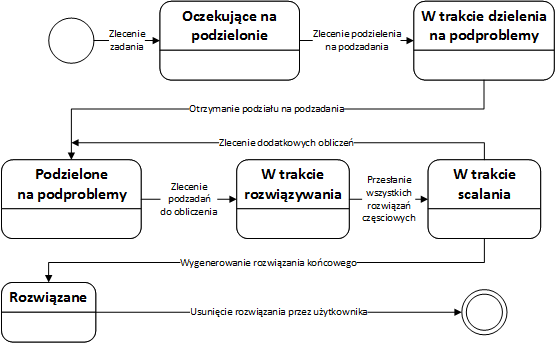
\includegraphics[width=\textwidth]{img/state/Task.png}
		\caption{Diagram stanów zadania}
	\end{figure}
	
	W celu optymalnego przechowywania zleconych przez użytkownika zadań opracowaliśmy
	strukturę ich przechowywania w której główny podział stanowi rodzaj problemu
	(TSP, DVRP itp.), a jego w obrębie znajdują się osobne listy FIFO dla nowo zgłoszonych problemów,
	podproblemów do rozwiązania oraz podproblemów do scalenia. Rodzaj problemu dla przyspieszenia obliczeń
	przechowywuje także informacje o menadżerach zadań i węzłach obliczeniowych, które potrafią
	go obsłużyć. 
	
	Serwer komunikacyjny w momencie wyboru zadania filtruje rodzaje problemów w poszukiwaniu takich,
	które są mają oczekujące zadania oraz są rozwiązywalne, czyli posiadają do dyspozycji wolny menadżer zadań 
	oraz mają zlecone jakieś zadanie. Spośród tych rodzajów wybieramy zadanie zlecone najwcześniej, by zachować
	oczekiwaną kolejność zajmowania się z zadaniami.
	
	Przy przydzielaniu podzadań dla poszczególnych węzłów komunikacyjnych postępujemy analogicznie.
	
	Rozwiązania podzadań odsyłamy do menadżera zadań w celu scalenia po otrzymaniu ich wszystkich. Menadżer
	po analizie odpowiedzi może zdecydować o wygenerowaniu rozwiązania końcowego lub zlecić podzadania dodatkowe
	i odłożyć końcową odpowiedź na termin późniejszy. 
	
	\begin{figure}[h]
		\centering
		\caption{Wybór zadania przez serwer komunikacyjny}
		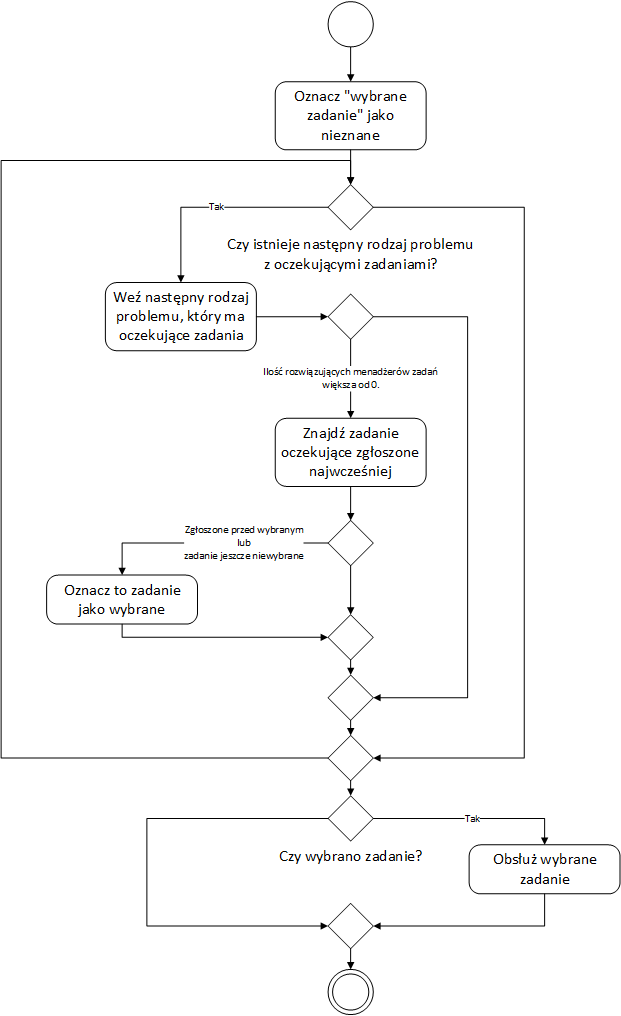
\includegraphics[width=\textwidth]{img/CommunicationServer-SelectTask.png}
	\end{figure}
	
\end{document}